\section{Scheibe}
    \subsection{Definition:}
        \begin{wrapfigure}[5]{r}{0.4\linewidth}
            \vspace{-5mm}
            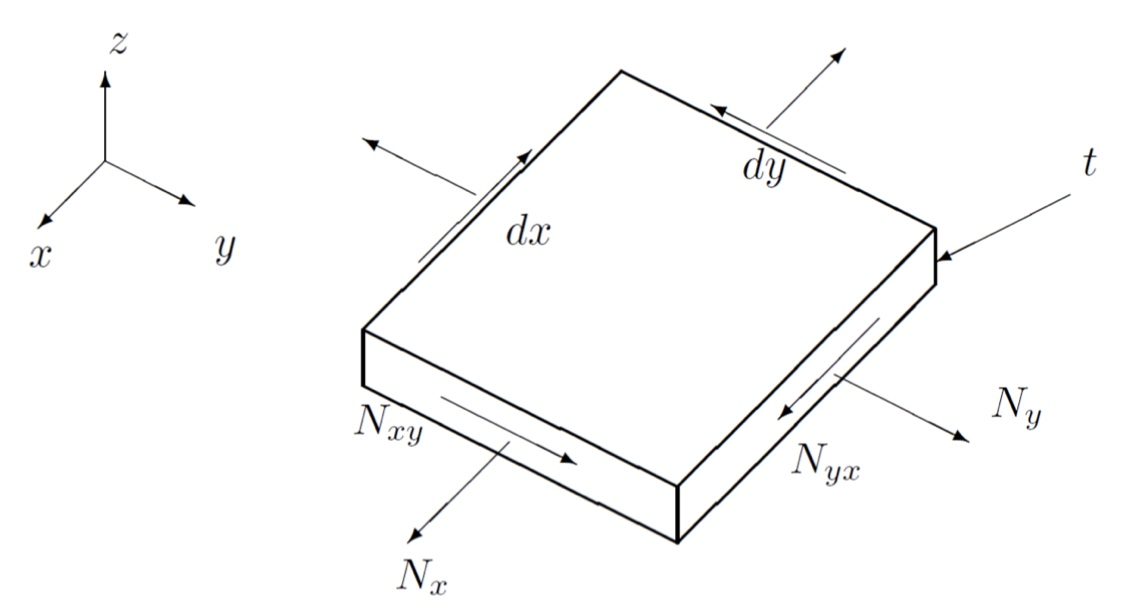
\includegraphics[width=\linewidth]{03/Scheibe}
        \end{wrapfigure}
        Scheibenelement: Dünnwandige Struktur mit Belastung in der Ebene. Äussere Kräfte dargestellt durch $N_x,N_y,N_{xy},N_{yx}$: Kräfte pro Längeneinheit ($\rightarrow$ Spannungen $\sigma_{xx},\sigma_{yy},\tau_{xy}$ über Dicke t integriert).\\
        
    \subsection{Annahmen:}
        \begin{enumerate}[noitemsep]
            \item Ebener Spannungszustand ($\sigma_{zz},\tau_{xz},\tau_{yz}=0$)
            \item Übrige Spannungskomponenten sind konstant verteilt in z-Richtung (homogene Spannungsverteilung)
            \item Keine Volumenkräfte
        \end{enumerate}
        1.,2.: Vernünftig, weil planare Dimensionen $\gg$ t \& keine Biegung. GGB reduziert sich zu:
        \[\sigma_{xx,x} + \tau_{xy,y}=0\quad\quad\sigma_{yy,y} + \tau_{xy,x}=0\]
        Definiere $F(x,y)$ (ayrische Spannungsfkt) mit $\sigma_{xx}=F_{,yy}$; $\sigma_{yy}=F_{,xx}$; $\tau_{xy}=-F_{,xy}$. Aus Kompatibilitätsbedingung: $\epsilon_{xx,yy}+\epsilon_{yy,xx}=2\epsilon_{xy,xy} \rightarrow \Delta\Delta F=0$ (Bi-potential Gleichung) Funktion F(x,y) so wählen, damit RB erfüllt.
        
    \subsection{Scheibe mit Loch:}

        \begin{itemize}
            \item Lochradius a $\ll$ L
            \item Belastung durch uniforme, einachsige Spannung S in grosser Entfernung vom Loch
            \item Spannungsfreie Rissflanken ($r = a; \forall\varphi\in\mathbb{R} $):\\ $\sigma_{rr}=0, \tau_{r\varphi}=0$
        \end{itemize}
        
        \begin{wrapfigure}[0]{r}{\linewidth}
            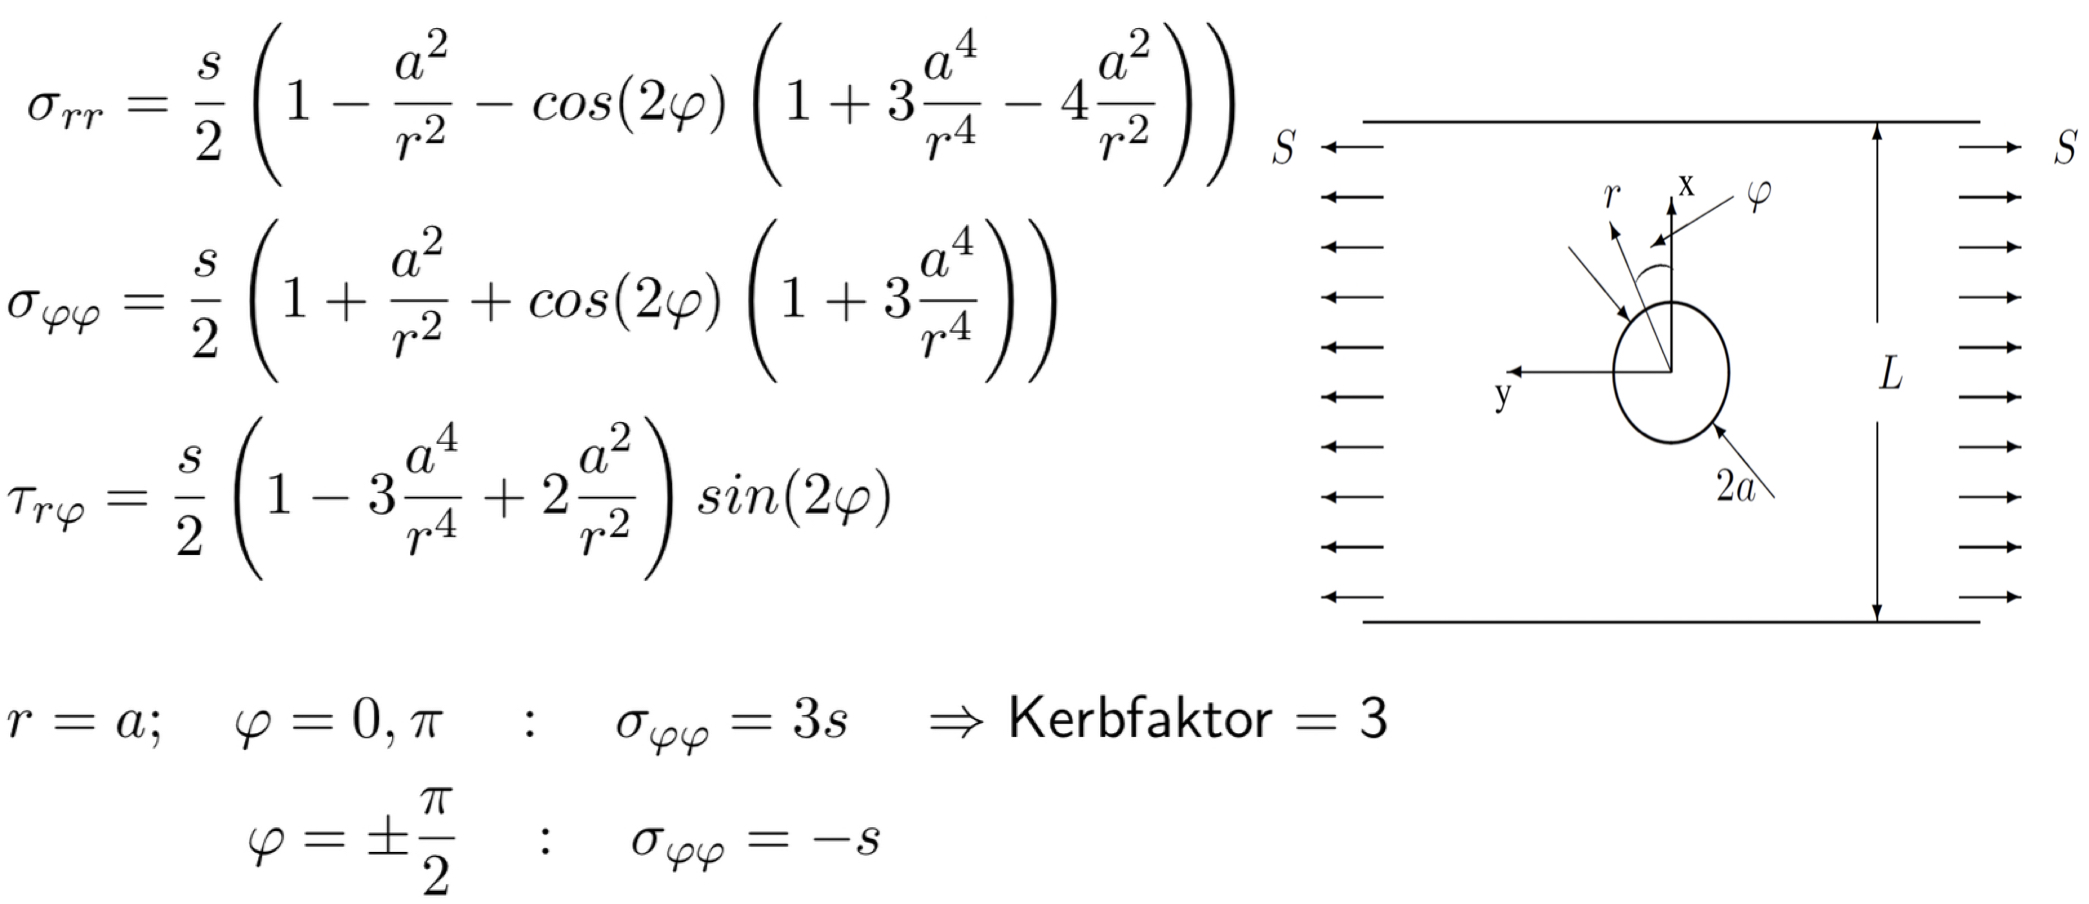
\includegraphics[width=\linewidth]{03/Scheibeloch}
        \end{wrapfigure}
        \begin{wrapfigure}[6]{r}{0.5\linewidth}
            \vspace{-10mm}
            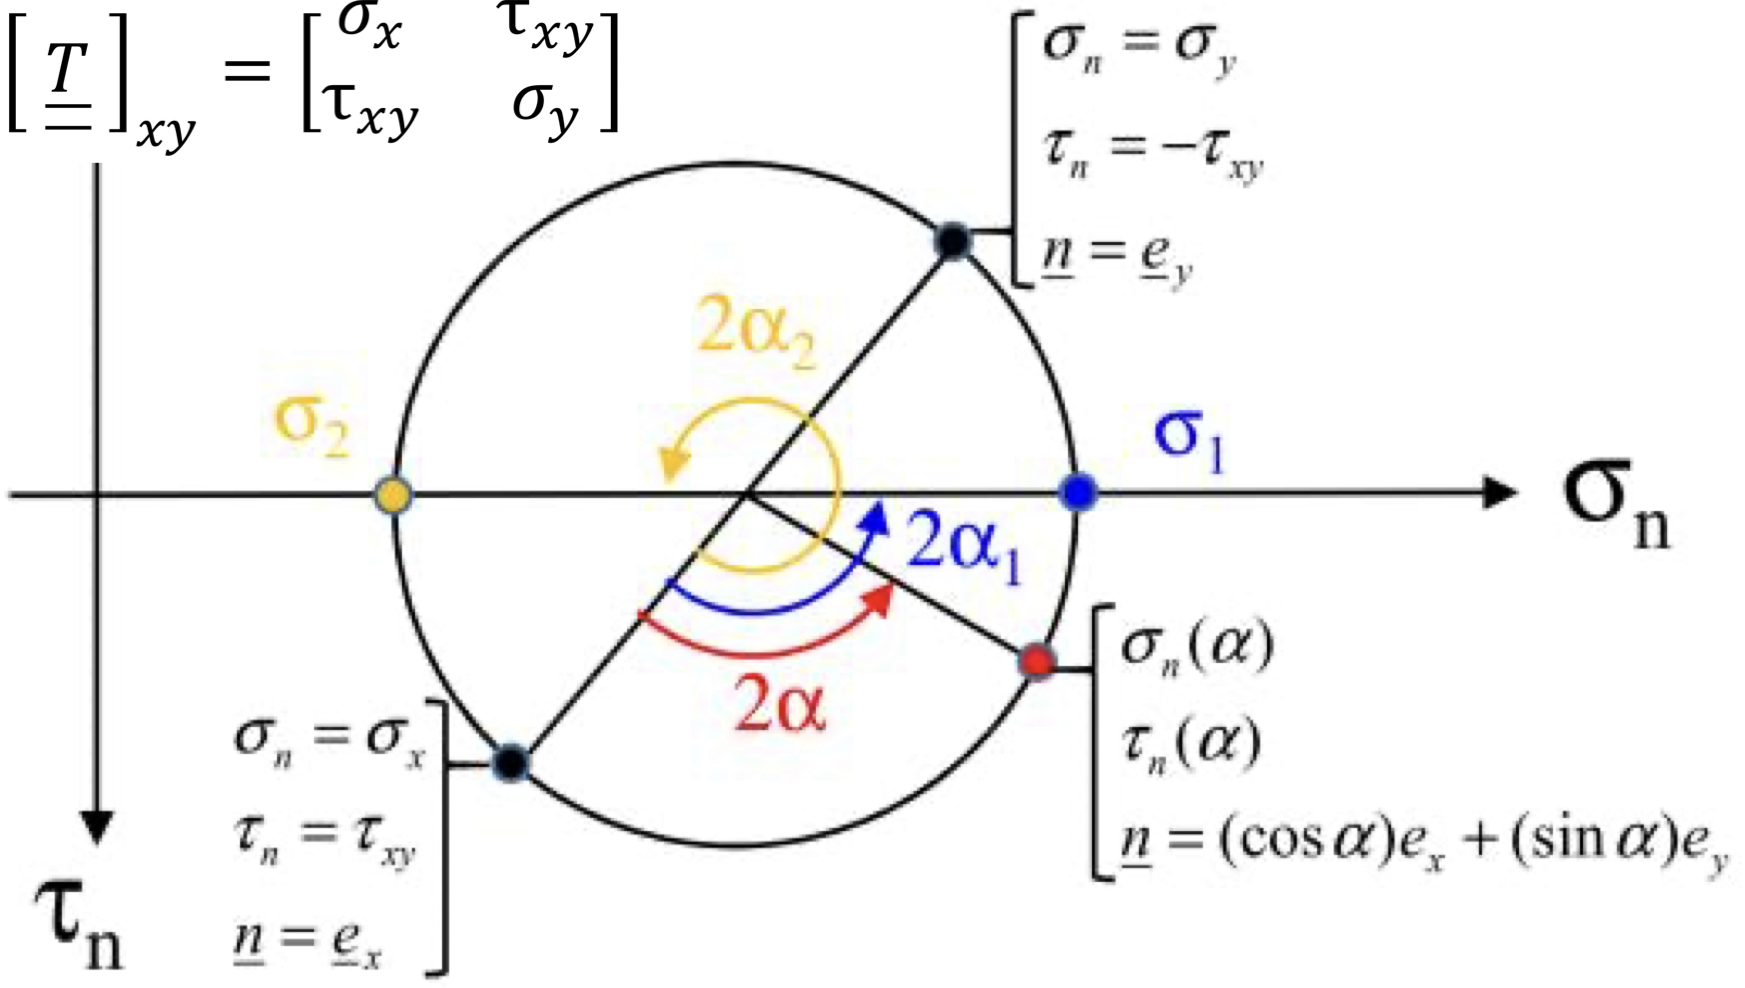
\includegraphics[width=\linewidth]{03/Mohrscher_Kreis.png}
        \end{wrapfigure}
        \textbf{Superposition} von mehreren Spannungen \& Spannungsrichtungen möglich. Bei Schubspannungen in Hauptspannungen umwandlen (Mohrscher Kreis).
        \\
        
    \subsection{Scheibe mit Riss:}
        Spannungsfreie Rissflanken ($\forall r, \varphi=\pm\pi$): $\sigma_{\varphi\varphi}=0, \tau_{r\varphi}=0$
        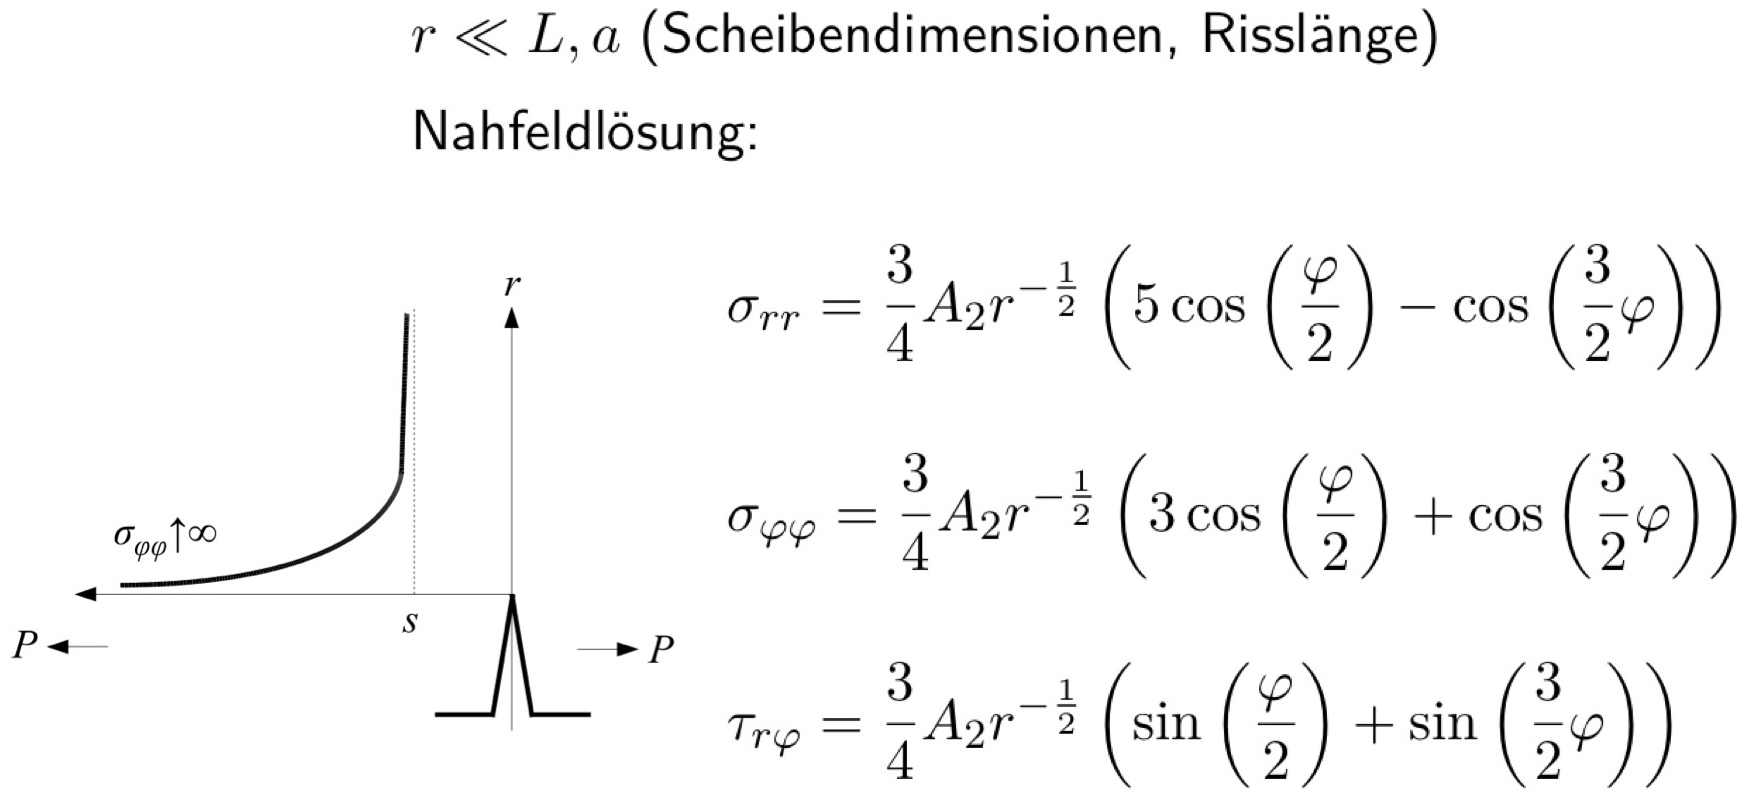
\includegraphics[width=70mm]{03/Scheiberiss}